\documentclass{article}
\usepackage[utf8]{inputenc}
\usepackage{graphicx}
\usepackage{svg}
% change reference style to [1], remove stupid sorting, language changed so date in ddmmyyyy
\usepackage[backend=biber, style=alphabetic, sorting=none, language=australian]{biblatex}
\addbibresource{References.bib}

\title{Report}
\author{David Saunders (910995)}
\date{April 2020}

\begin{document}
\maketitle

% \begin{abstract} 
%     Write abstract here. 4 page report!
% \end{abstract}

%\tableofcontents

\section{Introduction}
%10%
% Contextualise the machine-learning problem and introduce the
% task and the hypothesis. Make sure to include a few references to previous
% work. You should demonstrate an awareness of the research-area.

Image detection is a one of the most classic machine learning problem, with hundreds of papers on the topic.
Arguably the most influential paper on the topic ``Imagenet classification with deep convolutional neural networks'' showed how deep convolutional neural networks are considerably better at image classification than other methods.
The task of automatically playing a 3D game of PacMan poses a novel use of the technology.
From a starting position the points must be projected from 3D to 2D and scanned using image recognition to detect a series of 11 spheres located in a pointcloud.
Detection of pointclouds using deep learning methods is still a developing field so for this task the 2D image will be used \cite{guo2019deep}. 
The spacial coordinates of the sphere will be computed, and the position will be updated to that of the sphere.
That sphere will then be marked as collected, this process will then be repeated until all 11 spheres are collected.


% Maybe started with the MNIST handwritten digit classification problem.
% Is regarded by many as the ``Hello world'' of machine learning/CNNs \cite{tensorflow_2020}.
% History of image detection is relatively recent.

% One guy on kaggle used a cnn for the first time to great effect.
% Other more advanced problems such as image recognition, gesture
%     , emotion detection now possible thanks to deeper networks, and convolution's layers.
%https://towardsdatascience.com/deep-learning-for-image-classification-why-its-challenging-where-we-ve-been-and-what-s-next-93b56948fcef



% Maybe touch on the problem some people have of using too advanced method for the task?
% Especially with stuff like pretrained CNN specialised for facial recognition used to detect a black or white dot for example.
With machine learning there is a tendency to always use the newest and most complicated model when a simpler model may perform comparably \cite{forbes2020}.
This bias-variance tradeoff can be used to find a balance between the complexity of a model and its effectiveness, where more complicated models are not always more effective \cite{neal2018modern}.
Large complex neural networks can suffer from the problem of explainability.
It is common regard the inner workings as an unexplained ``black box'' \cite{zednik2019solving}.
Alternatively simple dummy classifiers are often used as a baseline to compare to other more advanced models \cite{dummyclassifier_2019}.

This report will design a relatively advanced CNN and a simpler dummy classifier.
Their effectiveness in completing the task will be compared.  

\section{Methodology}
%50%
% The model(s) you trained to undertake the task. Any decisions
% on hyperparameters must be stated here, including motivation for your
% choices where applicable. If the basis of your decision is experimentation
% with a number of parameters, then state this.                     The training data a classifier will be trained on has the size 51x51x3 where as t

The images obtained from the pointcloud have shape 160x240x3, where as the given training images have a different shape of 51x51x3.
This means that images from the pointcloud cannot directly be input into a classifier created from the given images.
Instead a sliding window approach will be used, to split larger image into windows the same size as the training data.
The windows will overlap strongly so that the set of windows will contain multiple partial spheres \cite{forsyth2002computer}.
We will attempt to train the classifiers so that it only recognises a sphere if it is in the centre of an image, therefore the centre pixel of the image will always be the depth.
The camera will then move to the sphere with the lowest depth, which will be the closest sphere.
The X,Y,Z coordinates of the sphere will be found from the middle pixel value for the projected mappings.
If no spheres are detected in any window then the viewpoint will rotate $-\frac{\pi}{6}$ radians in the Y axis until a sphere is detected.
This process will repeat until all spheres have been collected.

\subsection{Classifier 1: Convolutional Neural Network}

It was decided to use a Convolutional Neural Network (CNN) as a sphere classifier due to their tried and trusted effectiveness at image detection.
Detecting the red sphere is a trivial use of the technology so accuracy is expected to be very high.
%Problem will be with the training data not relating to the real life data where the spheres will be obscured and different sizes from the training.
%Problem of training/archived data not matching production is a well known issue (with prediction and stuff) TODO: ref.
A benefit of using a CNN is that we do not have to worry about feature extraction, the training data can be input directly into the network.

All of the architecture of the CNN will be explained in this section and all of the hyperparameters explained.
The CNN used in this task is similar to previous Imagenet classification CNN's where there are a series of convolutional and pooling layers
, followed by a fully connected layer \cite{krizhevsky2012imagenet}. 
The architecture used in this CNN is heavily inspired by the LeNet-5 Convolutional neural network, originaly used for handwritten digits recognition.
This architecture was chosen as it is one of the first CNN's to be proposed and it is relatively shallow compared to newer deep learning methods, so training time and memory usage will be less intensive \cite{lecun1998gradient}. 

\begin{figure}[ht]
    \noindent\makebox[\textwidth]
    {%
        \centering
        %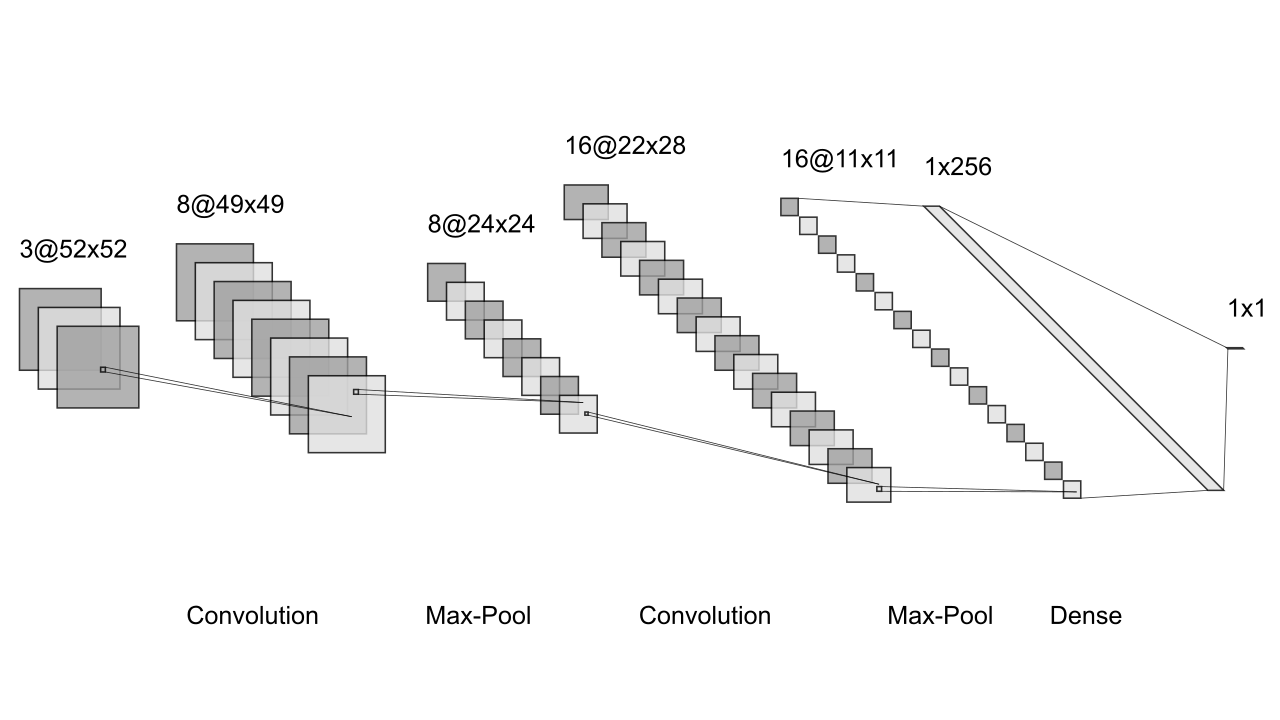
\includegraphics[scale=0.8]{CNN_Zoomed.png}
        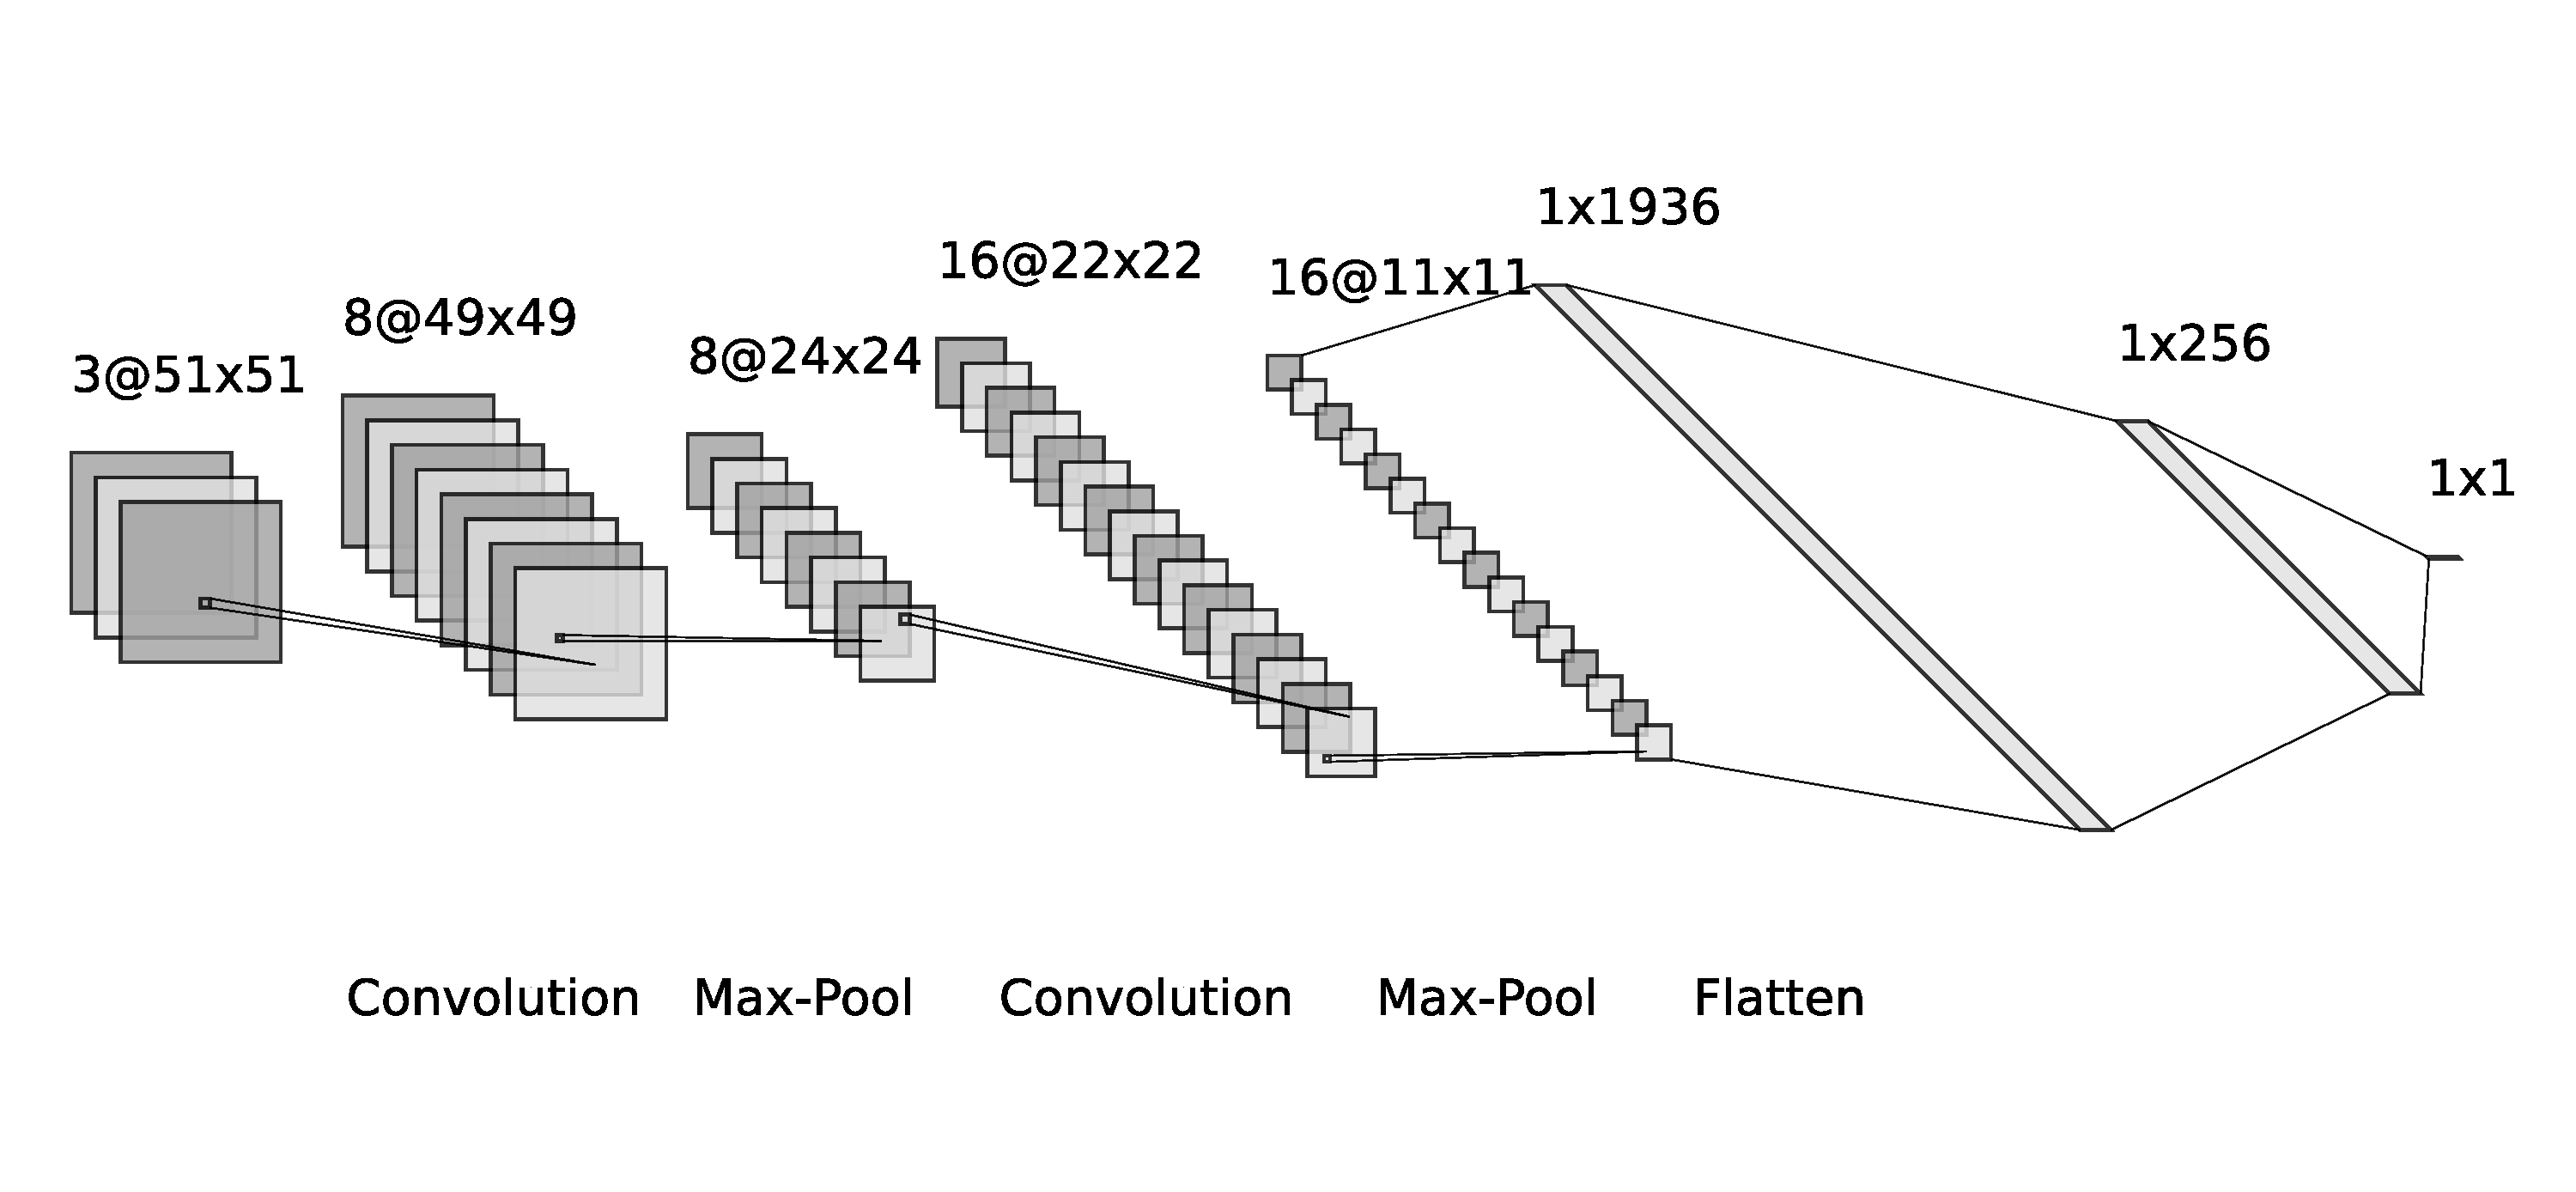
\includegraphics[scale=0.25]{CNN.pdf}
    }
    \caption{A diagram of the network showing the layers of the network designed for this task \cite{LeNail2019}.}
    \label{fig:diagram}
\end{figure}

Figure \ref{fig:diagram} shows the network consists of two convolutional layers
, which are then flattened and fed into  a dense fully connected layer
, which leads to a single output neuron.
Each convolutional layer is followed by a maxpooling layer, which is used to downsample the image.
It is hoped that max pooling will pick up any feature found by the earlier layers.
% TODO answer WHY maxpooling not another pooling method?
%Why max-pooling is used and not min pooling, or average pooling.
%Pooling size is 2, 2 WHY and what exactly does it mean?

% TODO: explain why relu was chosen? Activation of each internal layers use relu as that is default for whatever reason. Alternative is to use something like sigmoid, but relu is now generally used because xyz. 
All internal nodes of the network use the standard relu as the activation function, other than the single output neuron which uses the probability based sigmoid function.
The kernel size of the convolutional kernels were chosen arbitrarily as 3x3, and the pooling layers used are 2x2.
Due to the nature of kernel convolutions the input size of each layer will change slightly.
This will be detailed below.

The first convolutional layer takes in a 51x51x3 image, and outputs 8 filters with a reduced size of width and height of 49x49.
The filters are then max pooled to give a new shape of 24x24x8.
The second convolutional layer inputs the downsampled results and outputs a higher number of 16 filters.
The number of filters is increased in an attempt to group together any lower level features that have been identified.
Compared to other image classification tasks this one is trivial so there is no need for more layers to detect low and high level features.
Regardless when a shallower network was tried it didn't work so here we are.  
Pooling after this layer results in an output of shape 11x11x16.
After the convolutional layers we then flatten the output into a vector of length 1936 so that it can be input into a more traditional dense network of nodes.
A layer of 256 neurons is used as the hidden layer, which connects to a single neuron which predicts what class the input image belongs to.
This is given as a probability from 0 (no sphere present) to 1 (sphere present).
Between the hidden and output layers there is a dropout amount specified at 50\%, this means that half of these neurons randomly wont fire.
This method has been shown to reduce overfitting as each hidden neuron cannot rely on another neuron firing \cite{hinton2012improving}. %(weak explanation) 

When training the network the loss function is chosen to be binary crossentropy the CNN is predicting binary data.
The adaptive learning rate method Adam was chosen as optimizer as it has low memory requirements and works with little tuning of the hyperparameters \cite{Chengwei_2018}.
The data will be trained with 5 epochs, as this should maximise accuracy but prevent overfitting which is an issue with such a small dataset.
%machinelearningmastery.com/early-stopping-to-avoid-overtraining-neural-network-models/}
%This article list loads of nice academic sources about how to avoid overfitting.

% The model is then saved to disk as a $.hdf5$ file.
% This is so the networks weights doesn't have to be retrained all the time and to help reproducibility.
% (Get reference to why you should always save a model)
% Since networks are non-deterministic they may not always have the same result (ref).
The CNN will be used to classify a sphere only if there is a confidence of at least 99.9\% to avoid false positives. 

\subsection{Classifier 2: Dummy classifier}
A CNN should be able to detect a sphere, but could a simpler method complete the task just as effectively?
Feature engineering is the process of selecting features for a model using domain knowledge and some claim it is the most important factor to the success of a machine learning project \cite{domingos2012few}.
From the training data we can see that the centre pixel of a positive sample contains a high intensity for the red channel and low intensities for the green and blue channels.
Without using any machine learning methods a classifier was created that looks at the intensity of a single pixel and predicts if an image contains a sphere. 
A dummy classifier can be defined as ``a classifier that makes predictions using simple rules'' so that is what we wil call this classifier \cite{dummyclassifier_2019}.
If the classifier is successful then it will show using knowledge to extract features could prove just as effective as state of the art machine learning.
There may even be computational speedup benefits when a more simple method was used.

% while messing around it was found that multiple layers were needed to properly classify the spheres.
% Could manual feature engineering help? (Feature engineering is a good word just TODO: find reference.)
% In the training data the red sphere is always in the centre, with the center pixel having a very high red intensity, with a low intensity for the green and blue channels. 



\section{Results}
% 30%
% Describe, compare and contrast the results you obtained on your
% model(s). Any relationships in the data should be outlined and pointed
% out here. Only the most important conclusions should be mentioned in
% the text. By using tables and confusion-matrices to support the section,
% you can avoid describing the results fully.

The PacMan game was successfully completed when both methods of classification were used.
The main for loop of the program took approximately 16 minutes to complete, regardless as to whether the CNN or dummy classifier was used.

The accuracy of the CNN was 99.7\% (3.s.f) as expected from a powerful detection network.
Only 2 of the test images were falsely identified as negatives and there were no false positives.
The dummy classifier was surprisingly effective for such a simple classifier, with a comparable accuracy of 99.0\% (3.s.f). 
Similarly there were no false positives but a higher 6 false negatives.
The impact of false negatives in this task are mitigated by the sliding window algorithm.
Since a sphere appears in multiple windows the classifier has multiple chances for detection. 

% Despite the classifier not being the bottleneck, there was a notable speed increase.
% One possible explanation for the speedup is that the dummy, classifier is less robust and adaptable to change than the CNN.
% Sphere has to be directly in centre of screen for the dummy classifier, meaning less spheres were identified and so less images to process.
% %TODO: Look at results to see if this theory holds any weight at all.

The biggest bottleneck to the system is not the chosen classifier, but rather the function of projecting the point cloud to the 5 different maps which is very time intensive.
Any difference in time between the classifiers is unimportant to this task as the classifier does not significantly impact the time of the task. 

\section{Discussion and Conclusion}
% 10%
% Restate the task and hypothesis/-ses concisely.
% Reiterate the methods used. Describe the outcome of the experiment
% and the conclusion that you can draw from these results in respect of the
% hypothesis/-ses.

The task performed in this report was to create simple binary image classifier that was to be used in conjunction with other methods to play a game similar to PacMan, moving thorough 3D space.
The classifier was used in conjunction to a sliding window algorithm to to detect the presence of a red sphere in an image.
A CNN was used as they are known to be effective at image classification.
A simple dummy classifier was also created using manual feature engineering, which was found to perform the task just a well just as well as the more adveanced classifier.
This shows how there is not always a need for the most advance options and that given some knowledge of the problem
, manual feature engineering can be just as effective.

\printbibliography

\end{document}